\chapter{Related Works}

Your related works, and your purpose and contribution which must be different as below.

\section{Mhd Zulfikar Akram Nasution/ 1164081}
\subsection{Teori}
\begin{enumerate}
\item Binary Classification atau diartikan kedalam bahasa indonesia yaitu Klasifikasi Biner adalah tugas dalam mengklarifikasikan elemen-elemen dari himpunan yang diberikan kedalam dua kelompok berdasarkan aturan klarifikasi. Pada ummnya klarifikasi biner akan jatuh ke dalam domain Supervised Learning dan dimana kasus khusus hanya memiliki dua kelas.
\begin{itemize}
\item  Contoh Binary Classification pada gambar 2.1
\end{itemize}
\begin{figure}[ht]
\centering
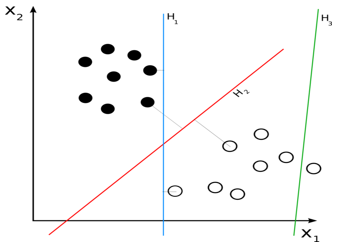
\includegraphics[scale=0.9]{figures/zulfikar/1.png}
\caption{Binary Classification}
\end{figure}

\item Supervised Learning, Unsupervised Learning, dan Clustering
\begin{itemize}
\item Supervised Learning
\end{itemize}
\par
Supervised learning adalah tugas pembelajaran mesin untuk mempelajari suatu fungsi yang memetakan input ke output berdasarkan contoh pasangan input-output. Ini menyimpulkan fungsi dari data pelatihan berlabel yang terdiri dari serangkaian contoh pelatihan. Dalam pembelajaran yang diawasi, setiap contoh adalah pasangan yang terdiri dari objek input (biasanya vektor) dan nilai output yang diinginkan (juga disebut sinyal pengawas). Contoh pada gambar 2.2
\begin{figure}[ht]
\centering
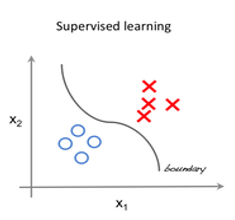
\includegraphics[scale=0.9]{figures/zulfikar/2.png}
\caption{Supervised Learning}
\end{figure}

\begin{itemize}
\item Unsupervised Learning
\end{itemize}
\par
Unsupervised Learning merupakan sebuah data yang belum ditentukan variabelnya jadi hanya berupa data saja. Dalam sebuah kasus Unsupervised Learning adalah aggap saja anda belum pernah membeli buku sama sekali dan pada suatu hari anda telah membeli buku dengan sangat banyak dalam kategori yang berbeda. Sehingga buku tersebut belum di kategorikan dan hanya berupa data buku saja. Coontoh seperti pada gambar 2.3
\begin{figure}[ht]
\centering
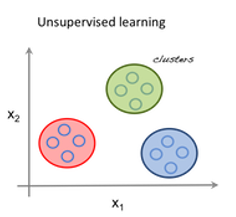
\includegraphics[scale=0.9]{figures/zulfikar/3.png}
\caption{Unsupervised Learning}
\end{figure}

\begin{itemize}
\item Clustering
\end{itemize}
\par
 Classtering merupakan sebuah proses untuk mengklasifikasikan sebuah data dalam satu parameter. Dalam kasus ini dapat dijelaskan ada beberapa orang yang memiliki kekuatan tubuh yang sehat dan kekuatan tubuh yang lemah. Parameter bagi orang yang memiliki tubuh yang kuat adalah orang yang terlihat bugar dan sehat maka dengan orang yang memiliki parameter adalah orang yang memiliki kekuatan tubuh yang kuat dan untuk kekuatan tubuh yang lemah adalah sebaliknya. Contoh seperti pada gambar 2.4
\begin{figure}[ht]
\centering
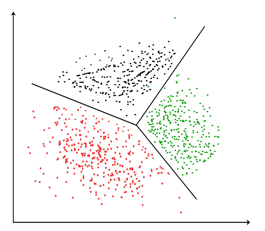
\includegraphics[scale=0.9]{figures/zulfikar/4.png}
\caption{Clustering}
\end{figure}

\item Evaluasi dan Akurasi
\par
 Evaluasi adalah tentang  bagaimana kita dapat mengevaluasi seberapa baik model bekerja dengan mengukur akurasinya. Dan akurasi akan didefinisikan sebagai persentase kasus yang diklasifikasikan dengan benar. Kita dapat menganalisis kesalahan yang dibuat oleh model, atau tingkat kebingungannya, menggunakan matriks kebingungan. Matriks kebingungan mengacu pada kebingungan dalam model, tetapi matriks kebingungan ini bisa menjadi sedikit sulit untuk dipahami ketika mereka menjadi sangat besar.

\item Cara Membuat dan Membaca Confusion Matrix
\begin{itemize}
\item Tentukan pokok permasalahan dan atributnya
\item Buat Decicion Tree
\item Buat Data Testing
\item Mencari nilai variabelnya misal a,b,c, dan d
\item Mencari nilai recall, percision, accuracy, dan error rate
\end{itemize}
\par contoh confusion matrix
	\begin{verbatim}
		Recall = 3/(1+3) = 0,75
		Percision = 3/(1+3 = 0,75
		Accuracy = (5+3)/(5+1+1+3) = 0,8
		Error Rate = (1+1)/(5+1+1+3) 0,2
	\end{verbatim}

\item Cara Kerja K-Fold Cross Validation
	\begin{itemize}
		\item Total instance dibagi menjadi N bagian.
		\item Fold yang pertama adalah bagian pertama menjadii testing data dan sisanya menjadi training data.
		\item Hitung akurasi berdasarkan porsi data tersebut dengan menggunakan persamaan.
		\item Fold yang ke dua adalah bagian ke dua menjadi testing data dan sisanya training data. 
		\item Hitung akurasi berdasarkan porsi data tersebut.
		\item Lakukan step secara berulang hingga habis mencapai fold ke-K.
		\item Terakhir hitung rata-rata akurasi K buah.
	\end{itemize}
\par
Berikut ilustrasi K-Fold Cross Validation seperti pada gambar 2.5
\begin{figure}[ht]
\centering
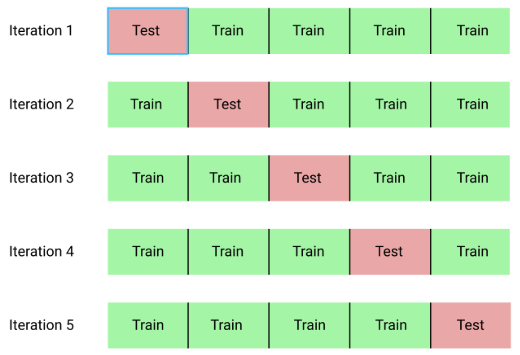
\includegraphics[scale=0.9]{figures/zulfikar/5.png}
\caption{K-Fold Cross Validation}
\end{figure}

\item Decision Tree
\par 
Decision Tree adalah sebuah metode pembelajaran yang digunakan untuk melakukan klarifikasi dan regresi. Decision Tree digunakan untuk membuat sebuah model yang dapat memprediksi sebuah nilai variabel target dengan cara mempelajari aturan keputusan dari fitur data. Contohnya seperti pada gambar 2.6 
\begin{figure}[ht]
\centering
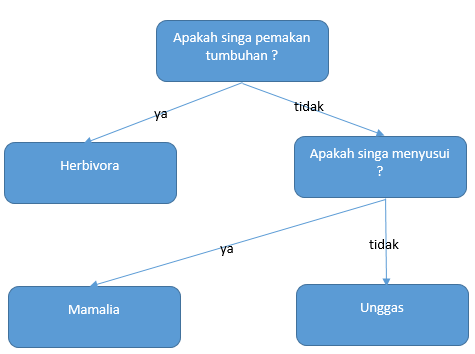
\includegraphics[scale=0.9]{figures/zulfikar/6.png}
\caption{Decision Tree}
\end{figure}

\item Gain dan Entropi
\begin{itemize}
\item Gain adalah pengurangan yang diharapkan dalam enthropy. Dalam mechine learning, gain dapat digunakan untuk menentukan sebuah urutan atribut atau memperkecil atribut yang telah dipilih. Urutan ini akan membentuk decision tree. atribut gain dipilih yang paling besar.
\item  Entropi adalah ukuran ketidakpastian sebuah variabel acak sehingga dapat di artikan entropi adalah ukuran ketidakpastian dari sebuah atribut.
\end{itemize}
\par Contoh seperti pada gambar 2.7
\begin{figure}[ht]
\centering
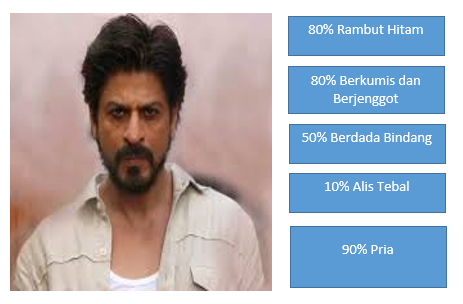
\includegraphics[scale=0.9]{figures/zulfikar/7.png}
\caption{Gain dan Entropi}
\end{figure}
\end{enumerate}

\section{Mhd Zulfikar Akram Nasution/ 1164081}
\subsection{Scikit-Learn}

\begin{enumerate}
\item
\begin{verbatim}
	# load dataset (student mat pakenya)
	import pandas as pd
	lontong    = pd.read_csv('student-mat.csv', sep=';')
	len(lontong)
\end{verbatim}
\begin{figure}[ht]
\centering
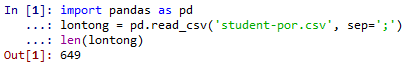
\includegraphics[scale=0.9]{figures/lontong/1.png}
\caption{Load Dataset}
\end{figure}
\par
	Codingan pertama ini akan meload ( menampilkan ) data pada file yang ditentukan. Untuk codingan ini file yang dieksekusi ialah " student-mat.csv " . Secara jelasnya, dalam codingan dapat dilihat bahwa variabel lontong didefinisikan untuk pembacaan csv dari " lontong " dimana untuk pemisahnya yaitu separation berupa ; . Setelah itu variabel lontong di "print" dengan perintah menampilkan "len" panjang ataupun jumlah dan hasilnya berupa angka 649 . 

\item
\begin{verbatim}
	# generate binary label (pass/fail) based on G1+G2+G3 
	# (test grades, each 0-20 pts); threshold for passing is sum>=30
	lontong['pass'] = lontong.apply(lambda row: 1 if (row['G1']+row['G2']+row['G3']) 
											>= 35 else 0, axis=1)
	lontong = lontong.drop(['G1', 'G2', 'G3'], axis=1)
	lontong.head()
\end{verbatim}
\begin{figure}[ht]
\centering
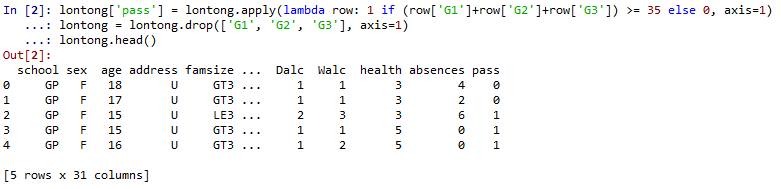
\includegraphics[scale=0.6]{figures/lontong/2.png}
\caption{Generate Binary Label}
\end{figure}
\par
	Codingan kedua ini secara keseluruhan menampilkan  baris  G1, G2 dan G3 ( berdasarkan kriterianya ) untuk kolom PASS pada variabel lontong. Untuk lebih jelasnya, pada codingan terdapat pendefinisian pembacaan "lambda" ( panjang gelombang ) dari baris G1, G2 dan G3. Apabila row-row tersebut bernilai lebih dari 35 maka akan terdefinisikan angka "1" apabila tidak, maka akan terdefinisikan angka "0" pada kolom PASS ( sesuai permintaan awal ). Selanjutnya variabelnya di "print" sehingga menampilkan keluaran. Tidak lupa terdapat juga jumlah dari baris dan kolom yang terubah sesuai dengan baris yang dieksekusi.


\item
\begin{verbatim}
	# use one-hot encoding on categorical columns
	lontong = pd.get_dummies(lontong, columns=['sex', 'school', 'address', 
									'famsize', 
									'Pstatus', 'Mjob', 'Fjob', 
	                               'reason', 'guardian', 'schoolsup', 
								   'famsup', 'paid', 'activities',
	                               'nursery', 'higher', 'internet', 
									'romantic'])
	lontong.head()
\end{verbatim}
\begin{figure}[ht]
\centering
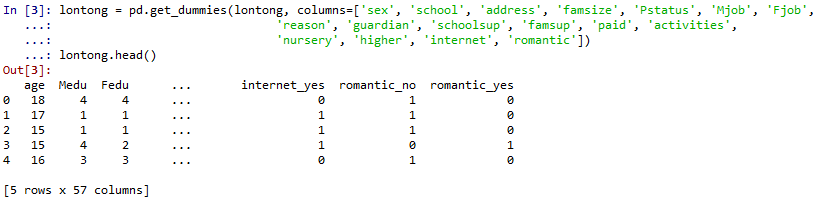
\includegraphics[scale=0.6]{figures/lontong/3.png}
\caption{Pemanggilan get dummies dari lontong}
\end{figure}
\par
	Secara keseluruhan, codingan ini mendefinisikan pemanggilan get dummies ke dalam variabel lontong. Di dalam get dummies sendiri akan terdefinisikan variabel lontong dengan kolom-kolom yang akan dieksekusi seperti school, address dll. Kemudian variabel tersebut di definisikan untuk mendapatkan kembalian berupa keluaran dari eksekusi perintah variabel lontong beserta dengan jumlah baris dan kolom data yang dieksekusi.

\item
\begin{verbatim}
	# shuffle rows
	lontong = lontong.sample(frac=1)
	# split training and testing data
	lontong_train = d[:500]
	lontong_test = d[500:]

	lontong_train_att = lontong_train.drop(['pass'], axis=1)
	lontong_train_pass = lontong_train['pass']

	lontong_test_att = lontong_test.drop(['pass'], axis=1)
	lontong_test_pass = lontong_test['pass']

	lontong_att = lontong.drop(['pass'], axis=1)
	lontong_pass = lontong['pass']

	# number of passing students in whole dataset:
	import numpy as np
	print("Passing: %d out of %d (%.2f%%)" % (np.sum(lontong_pass), len(lontong_pass), 
	       100*float(np.sum(lontong_pass)) / len(lontong_pass)))
\end{verbatim}
\begin{figure}[ht]
\centering
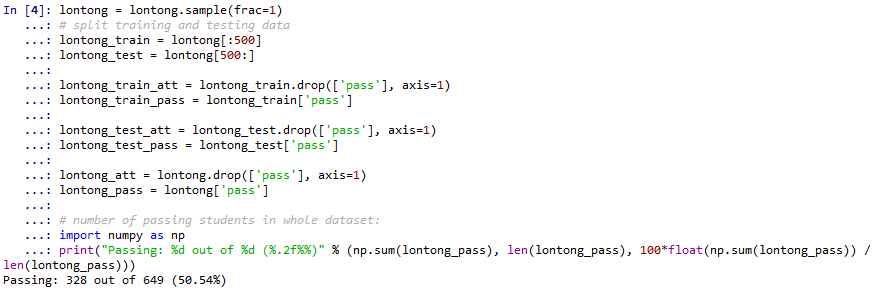
\includegraphics[scale=0.6]{figures/lontong/4.png}
\caption{Mendefinisikan pembagian data}
\end{figure}
\par
	Secara keseluruhan codingan ini difungsikan untuk mendefinisikan pembagian data yang berupa training dan testing data. Secara jelasnya pertama-tama variabel lontong akan mendefinisikan sampel yang akan digunakan ( berupa shuffle row ) . Nah kemudian masing2 parameter yaitu lontong train dan lontong test akan berjumlah 500 data ( telah dibagi untuk training dan testing ). Selanjutnya dilakukan pengeksekusian untuk kolom Pass, apabila sesuai dengan "axis=1" maka eksekusi fungsi berhasil. Selain itu juga disertakan jumlah dari peserta yang lolos dari semua nilai data setnya.

\item 
\begin{verbatim}
	# fit a decision tree
	from sklearn import tree
	soto = tree.DecisionTreeClassifier(criterion="entropy", max_depth=5)
	soto = soto.fit(lontong_train_att, lontong_train_pass)
\end{verbatim}
\begin{figure}[ht]
\centering
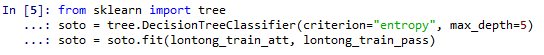
\includegraphics[scale=0.9]{figures/lontong/5.png}
\caption{Membuktikan pengujian}
\end{figure}
\par
	Secara keseluruhan, codingan ini hanya membuktikan pengujian dari Klasifikasi Decision Tree yang ada, apakah true atau tidak dan hasilnya true. Apabila dibahas secara lengkap maka pada codingan ini di definisikan library sklearn untuk mengimpor atau menampilkan tree. Variabel soto difungsikan untuk membaca klasifikasi decision tree dari tree itu sendiri dengan 2 parameternya yaitu kriteria="entropy" dan max depth=5. Maka selanjutnya variabel soto akan masuk dan terbaca dalam module fit dengan 2 parameter yaitu lontong trai att dan lontong train pass.

\item
\begin{verbatim}
	# visualize tree
	import graphviz
	dot_data = tree.export_graphviz(soto, out_file=None, label="all", 
									impurity=False, proportion=True,
	                                feature_names=list(lontong_train_att), 
									class_names=["fail", "pass"], 
	                                filled=True, rounded=True)
	graph = graphviz.Source(dot_data)
	graph
\end{verbatim}
\begin{figure}[ht]
\centering
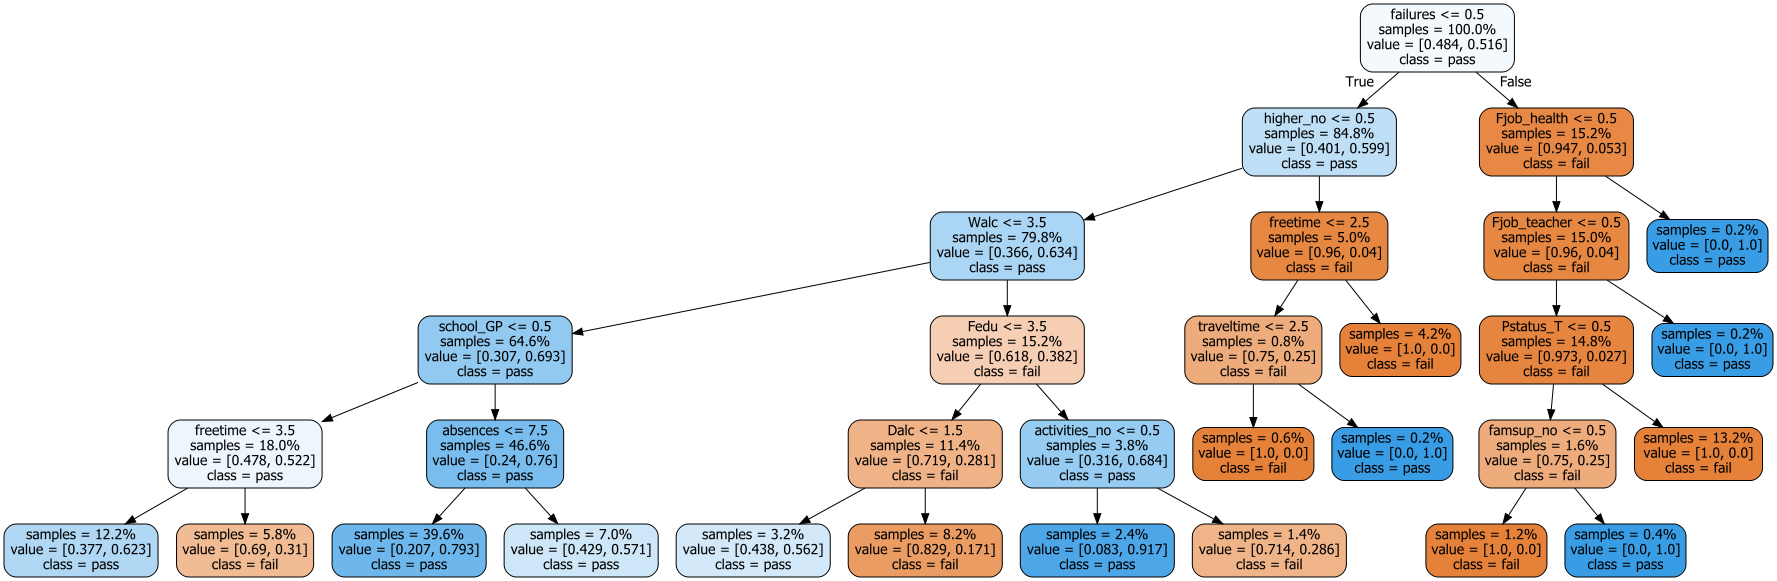
\includegraphics[scale=0.3]{figures/lontong/6.png}
\caption{Gambaran decision tree}
\end{figure}
\par
	Codingan ini memberikan gambaran dari klasifikasi decision tree dari pengolahan parameter yang dieksekusi kedalam variabel soto. Tentunya dengan pemanfaatan library graphviz yang telah diimport dan difungsikan.

\item
\begin{verbatim}
	# save tree
	tree.export_graphviz(soto, out_file="student-performance.dot", 
						 label="all", impurity=False, 
						 proportion=True,
	                     feature_names=list(lontong_train_att), 
	                     class_names=["fail", "pass"], 
	                     filled=True, rounded=True)
\end{verbatim}
\begin{figure}[ht]
\centering
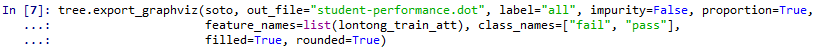
\includegraphics[scale=0.6]{figures/lontong/7.png}
\caption{Library Graphviz}
\end{figure}
\par
	Pada gambar 7 akan menampilkan yang terdapat pada Library Graphviz, apabila benar akan menampilkan hasil output seperti yang terdapat pada gambar.

\item
\begin{verbatim}
	soto.score(lontong_test_att, lontong_test_pass)
\end{verbatim}
\begin{figure}[ht]
\centering
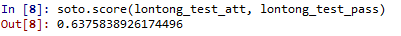
\includegraphics[scale=0.9]{figures/lontong/8.png}
\caption{Menampilkan hasil perhitungan 2 parameter}
\end{figure}
\par
	Menampilkan hasil perhitungan dari kedua parameter yang terdapat pada code tersebut. Yang merupakan perhitungan hasil prediksi silang akan kemungkinan nilai di masa mendatang.

\item
\begin{verbatim}
	from sklearn.model_selection import cross_val_score
	kari = cross_val_score(soto, lontong_att, lontong_pass, cv=5)
	# show average score and +/- two standard deviations away 
	#(covering 95% of scores)
	print("Accuracy: %0.2f (+/- %0.2f)" % (kari.mean(), kari.std() * 2))
\end{verbatim}
\begin{figure}[ht]
\centering
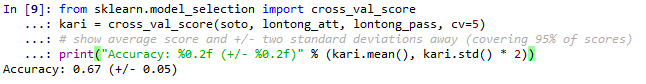
\includegraphics[scale=0.6]{figures/lontong/9.png}
\caption{Mendefinisikan library sklearn}
\end{figure}
\par
	Kodingan tersebut mendefinisikan library sklearn model selection dan import cross val score. Dan kemudian variabel kari mengeksekusi fungsi cross val score(soto, lontong att, lontong pass, cv=5). Kemudian akan menampilkan nilai dari fungsi akurasinya.

\item 
\begin{verbatim}
	for max_depth in range(1, 20):
	    soto = tree.DecisionTreeClassifier(criterion="entropy", 
			max_depth=max_depth)
	    kari = cross_val_score(soto, lontong_att, lontong_pass, cv=5)
	    print("Max depth: %d, Accuracy: %0.2f (+/- %0.2f)" % 
				(max_depth, kari.mean(), kari.std() * 2)
			 )
\end{verbatim}
\begin{figure}[ht]
\centering
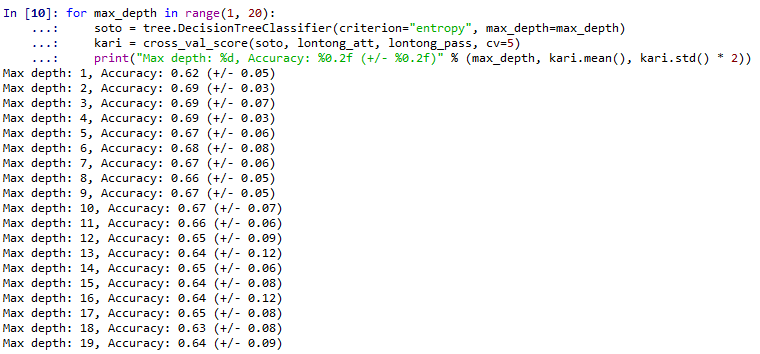
\includegraphics[scale=0.6]{figures/lontong/10.png}
\caption{Menampilkan hasil fungsi max depth dan accuracy}
\end{figure}
\par
	Pada gambar di atas kodingan nya berfungsi untuk menampilkan hasil dari fungsi Max Depth dan Accuraccy dari dari Decission Tree. Yaitu menmpilkan data dari angka 1-20.

\item
\begin{verbatim}
	depth_acc = np.empty((19,3), float)
	i = 0
	for max_depth in range(1, 20):
	    soto = tree.DecisionTreeClassifier(criterion="entropy", 
			max_depth=max_depth)
	    kari = cross_val_score(soto, lontong_att, lontong_pass, cv=5)
	    depth_acc[i,0] = max_depth
	    depth_acc[i,1] = kari.mean()
	    depth_acc[i,2] = kari.std() * 2
	    i += 1

	depth_acc
\end{verbatim}
\begin{figure}[ht]
\centering
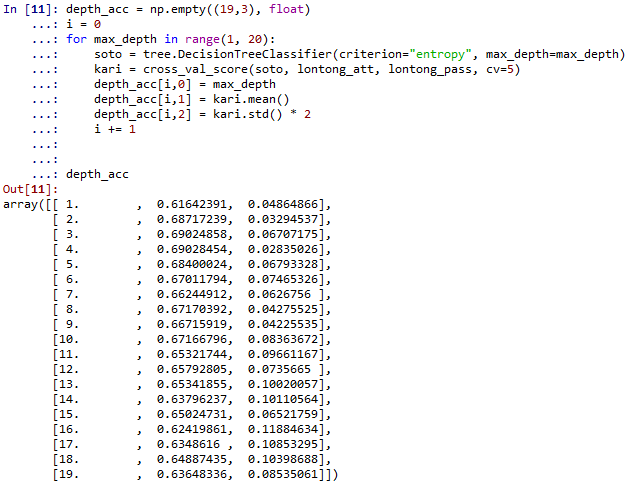
\includegraphics[scale=0.6]{figures/lontong/11.png}
\caption{Menjelaskan variable kari}
\end{figure}
\par
	Dijelaskan bahwa variable kari akan menampilkan atau mendefinisikan nilai dari variabel score yang mana isi dari variable score yaitu soto, lontong att, lontong pass, cv=5. Yang mana hasil tampilan dari kodingannya adalah outputan seperti gambar 11.

\item 
\begin{verbatim}
	import matplotlib.pyplot as plt
	fig, ax = plt.subplots()
	ax.errorbar(depth_acc[:,0], depth_acc[:,1], yerr=depth_acc[:,2])
	plt.show()
\end{verbatim}
\begin{figure}[ht]
\centering
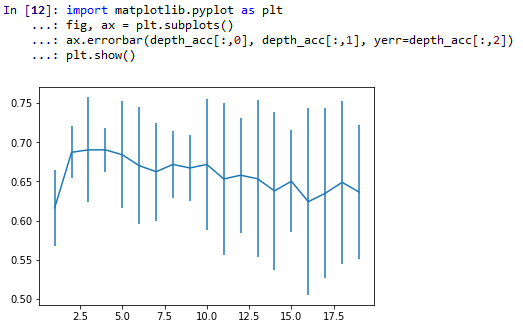
\includegraphics[scale=0.5]{figures/lontong/12.png}
\caption{Menjelaskan dan menampilkan gambar grafik}
\end{figure}
\par
	Pada gambar di atas dijelaskan bahwa pada library matplotlib akan menampilkan gambar grafik pada gambar 12 dari eksekusi fungsi ax.errorbar.

\end{enumerate}


\section{Penanganan Error}
Dari percobaan yang dilakukan di atas, error yang kita dapatkan di dokumentasikan dan di selesaikan(nilai 5 hari kedua):

\begin{enumerate}
	\item
ScreenShoot Error
\begin{figure}[ht]
\centering
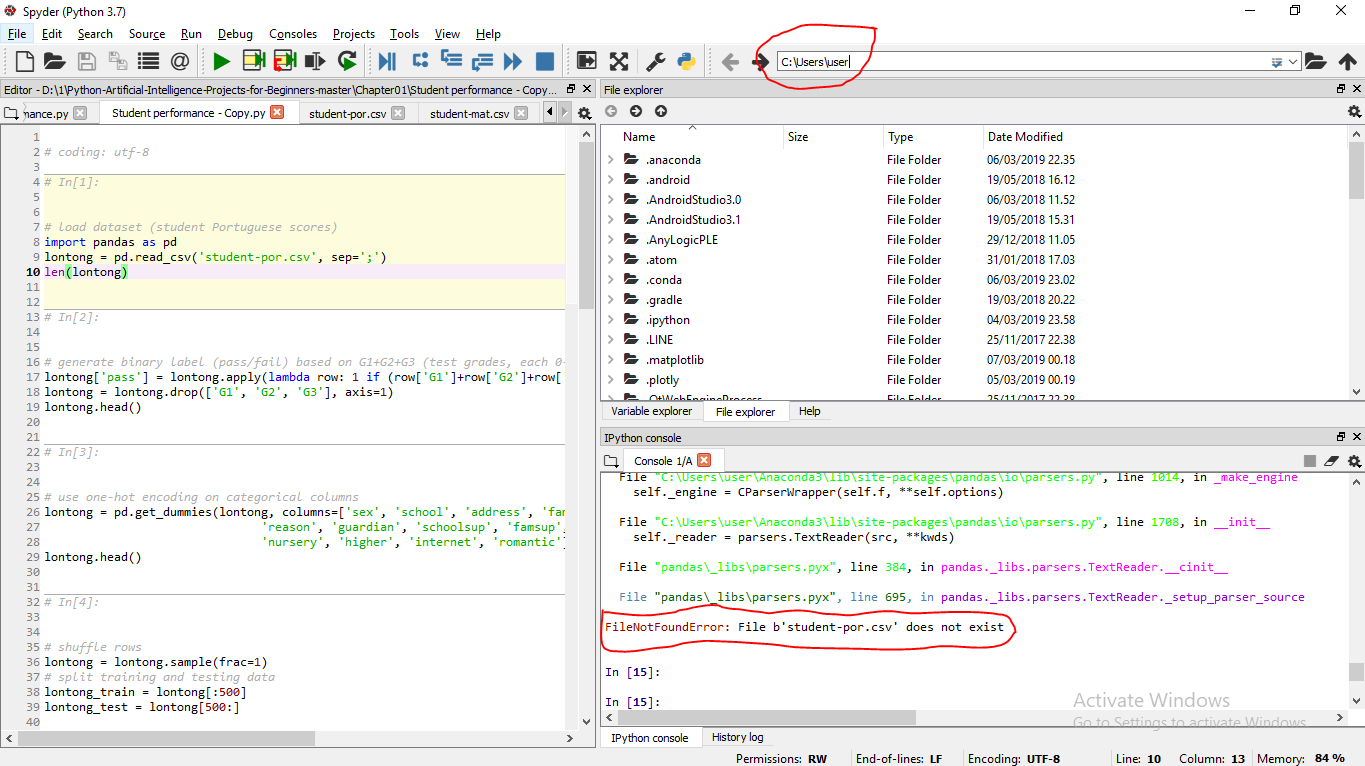
\includegraphics[scale=0.3]{figures/lontong/13.png}
\caption{ScreenShoot Error}
\end{figure}
	\item
Tuliskan kode eror dan jenis errornya
\par
Error ini disebabkan karena pada direktori C tidak terdapat file tersebut. 
	\item
Solusi pemecahan masalah error tersebut
\begin{itemize}
\item 	Masuk ke folder dimana file dataset berada, dapat dilihat dibawah ini
\item 	Setelah diganti, jalankan kembali skrip tersebut pasti akan berhasil
\end{itemize}
\begin{figure}[ht]
\centering
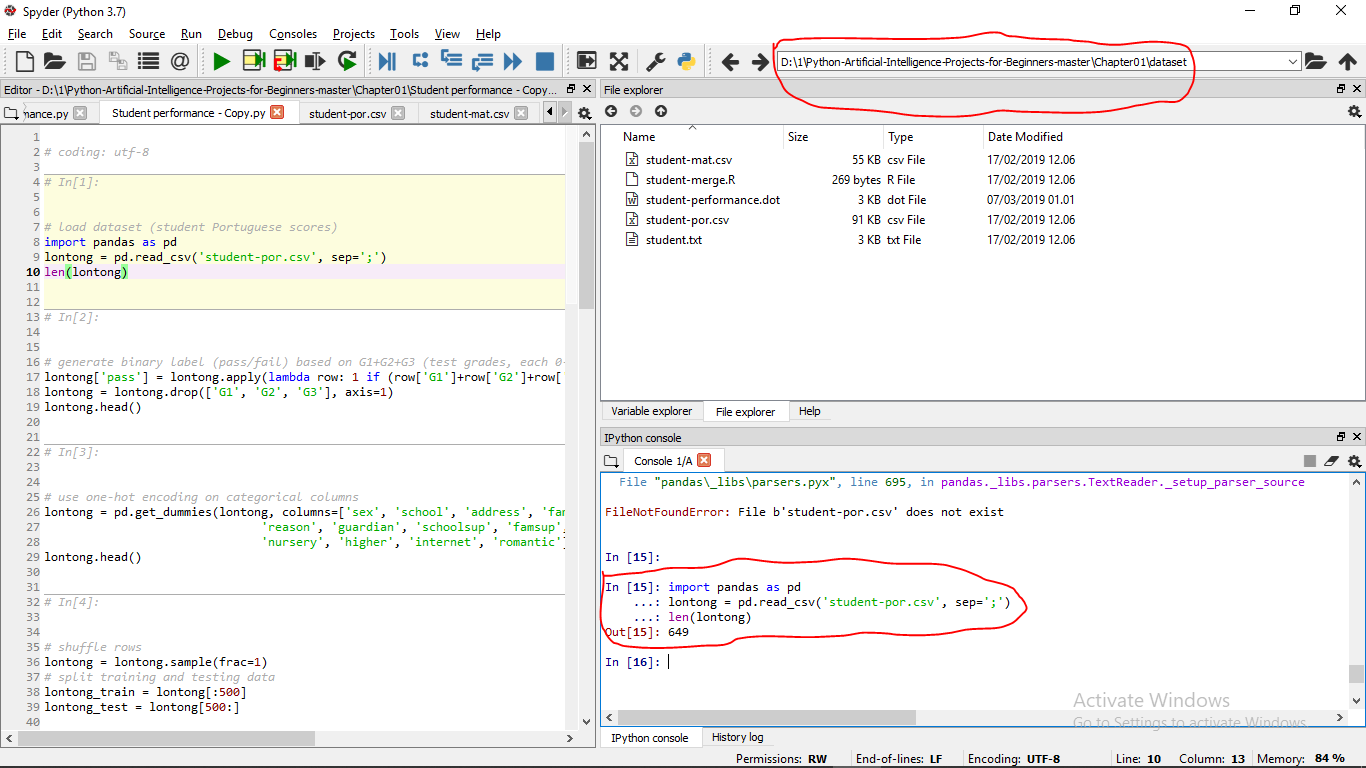
\includegraphics[scale=0.3]{figures/lontong/14.png}
\caption{Penanganan Error}
\end{figure}

\end{enumerate}

\section{Same Topics}
Cite every latest journal with same topic
\subsection{Topic 1}
cite for first topic

\subsection{Topic 2}
if you have two topics you can include here to


\section{Same Method}
write and cite latest journal with same method

\subsection{Method 1}
cite and paraphrase method 1

\subsection{Method 2}
cite and paraphrase method 2 if you have more method please add new subsection.

 